\documentclass[a4paper]{article}

\usepackage{graphicx}
\usepackage{amsmath}
\usepackage{a4wide}
% booktabs is here because the pandas generated latex tables use \toprule,
% \midrule, etc
\usepackage{booktabs}

\title{Identification of open loop dynamics of a manual controlled bicycle-rider system
}
\author{Jason K. Moore and Mont Hubbard}
\date{\today}

\begin{document}
n
\maketitle

\section{Introduction}

Today's experiments are capable of delivering a staggering amount of
both kinematic and kinetic data from complex dynamical systems. Such a large
amount of data lends itself to data driven modeling approaches that can
potentially provide more predictive models than first principles models. These data
driven models can also give insight into the deficiencies of first principles
models. Here we explore the bicycle-rider system with data driven modelling.

The bicycle/motorcycle-rider system has been described with a variety of
models. Many
studies of bicycles rely on the benchmarked Whipple model \cite{Meijaard2007},
with or without the addition of tire models, for analytical studies of the
system and simulation comparisons. The Whipple bicycle model \cite{Whipple1899}
is regarded as a highly predictive, yet ``simple'', model of the bicycle-rider
system and is constructed from first principles, yet very little experimental
data proves it robustly predicts bicycle-rider open
loop dynamics. The benchmarked Whipple 
model \cite{Meijaard2007} is minimal within an analytic framework that describes essential features such
as speed dependent stability, steer and roll coupling, and non-minimum phase
behavior.

We are aware of only three significant attempts to validate the
Whipple bicycle model with experimental data. The most cited
\cite{Kooijman2008,Kooijman2009} show that the Whipple model is predictive of
a \emph{riderless} bicycle in a gymnasium and on a treadmill for speeds in its
predicted stable speed range, 4-6 m/s. The other \cite{Cain2012} shows that
the Whipple model linearized in a steady turn predicts kinematics
but not the rider's applied steering torque. Open loop motorcycle-rider system dynamics have been 
identified  \cite{Eaton1973} and \cite{James2002,James2005}. Eaton
used frequency domain identification techniques, known to be problematic for closed loop identification \cite{Ljung1999}.
James showed that identified ARX models with lower order than typical first
principles models can predict the measured motion, but did not find very good
agreement with his high order first principles models.

We have collected a large set of
time history data from an instrumented bicycle under manual control. The
measurements include the most important kinematic and kinetic variables
describing bicycle-rider motion from three riders on the same
bicycle for a variety of maneuvers and speeds. These experiments generated
approximately 1.7 million time samples from about 30 sensors sampled at
200 hertz (about 2.4 hours of real time).

There is good reason to question some of assumptions in the Whipple model, namely knife-edge 
no-slip wheels, especially
under full rider weight. In addition, rider biomechanics have a larger
influence on and coupling to the bicycle than the motorcycle. Our identified models 
attempt to account for these and other discrepancies.

\section{Instrumented Bicycle Experiments}

We instrumented a bicycle with a unique combination of dynamic sensors. 
Rider biomechanical movement, including pedaling, was
    restricted to make the Whipple rigid-rider
    assumption more applicable and the bicycle was propelled by an electric
motor, Figure
\ref{fig:instrumented-bicycle} 
Experiments were performed both on the open road and on a treadmill.
Rear frame 3D angular rates
and a 3D point acceleration were measured with a VectorNav
VN-100 inertial measurement unit; rear frame roll angle with a
rotary potentiometer on a lightweight trailer; steer angle
using a rotary potentiometer; axial torque in the steer tube with
a Futek 150 in-lb (±17 Nm) TFF350 torque sensor; lateral seat-post perturbation force
by a 100 lb load cell (Interface SSM-100); inertial angular rate
of the front frame about the steer axis by a single axis rate gyro
(Silicon Sensing CRS03-04S); and rear wheel angular rate by a DC generator.
See \cite{Moore2012} for full details of the equipment.

\begin{figure}
  \label{fig:instrumented-bicycle}
  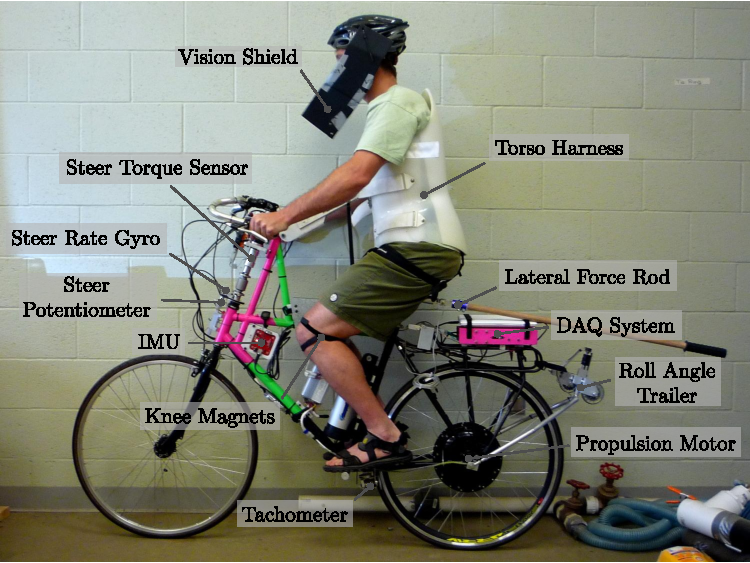
\includegraphics[width=5in]{figures/instrumented-bicycle.pdf}
  \caption{The instrumented bicycle with rider L seated in the harness.}
\end{figure}

The analysis herein focuses on two maneuvers we call \emph{Heading
Tracking} and \emph{Lateral Deviation Tracking}. During heading tracking the
rider was instructed simply to balance the bicycle and keep a relatively
constant heading while focusing their vision at a point in the distance.
During lateral deviation tracking the rider focused on a
straight line marked on the ground and attempted to keep the front
wheel on this line. Both tasks were performed with and without manually
applied lateral perturbation forces just below the seat,
random in direction and time during the trials. Each maneuver was
performed on both a 1 meter wide treadmill and an open gymnasium floor\cite{Moore2012}.


Physical parameters (geometry, mass, center of mass, and moments of
inertia) of both bicycle and rider were estimated using the methods in
\cite{Moore2012} and \cite{Yeadon1990}. Bicycle geometry was measured to get
accurate estimates of the parameters used in the benchmark model,
\cite{Meijaard2007}. Combined inertial properties of the bicycle rear frame
and rider were computed with standard methods. Two open source software
packages, \verb|yeadon| \cite{Dembia2011} and \verb|BicycleParameters|
\cite{Moore2011} manage and process the physical parameter data.

Before each day of testing, base data were collected for the system's sensors
for calibration purposes. Then for each trial a set of meta data and raw time
series were collected from the bicycle's onboard DAQ system. This data was
stored in a HDF5 database for easy querying and retrieval in the data analysis
step. Raw data was then processed to obtain the desired time histories
defined by the Whipple model coordinates, described in Table
\ref{tab:measurements}.

\begin{table}
  \centering
  \caption{The fundamental measurements from the instrumented bicycle.}
  \label{tab:measurements}
  \begin{tabular}{lll}
    \hline
    Variable                                            & Description                                    & Units \\
    \hline
    $v$                                                 & wheel center speed magnitude                   & m/s \\
    $\delta,\phi,\psi$                                  & steer, roll and yaw angles                     & rad \\
    $\dot{\delta},\dot{\phi},\dot{\psi},\dot{\theta}_B$ & steer, roll, yaw, and rear wheel angular rates & rad/s \\
    $T_\delta,F_{c_l}$                                  & steer torque, lateral perturbation force       & NM, N
  \end{tabular}
\end{table}

Signals were measured and processed as described in \cite{Moore2012}. Roll and 
steer accelerations were estimated by numerically differentiating
roll and steer rate signals. Before identification computations we subtracted
the temporal means of the signals that were generally symmetric about zero,
i.e. all but lateral force and speed. Then all signals were filtered
with a second order low pass Butterworth filter at a 15 Hz cutoff frequency.
Experimental data was collected on seven days and comprised
about 600 individual trials with three riders. We used 374 of the
runs for the following analysis.

% TODO: example plot of the signals
% TODO : add where to get the data

\section{Identification}
\label{sec:identification}

% TODO : This needs to be reworded to reflect that canoncial id

The linear Whipple model is a 4th order system with roll angle $\phi$, steer
angle $\delta$, roll rate $\dot{\phi}$, and steer rate $\dot{\delta}$ selected
as the independent states and with roll $T_\phi$ and steer $T_\delta$ torques
as the generalized forces and system inputs. In place of the roll torque input,
we extend the model to include a lateral force $F$ acting at a point on the
frame to provide a new input, accurately modelling imposed lateral
perturbations \cite{Moore2012}.  We also examine a second
candidate model which adds the inertial effects of the rider's arms to the
Whipple model, also described in \cite{Moore2012}. This model was designed to
more accurately account for the fact that the riders were free to move their
arms with the front frame of the bicycle. This model is similar to
the upright rider in \cite{Schwab2010}, but with slightly different joint
definitions. Constraints are chosen so that no additional degrees of freedom
are added, keeping the system both tractable and comparable to the benchmarked
Whipple model.

We make the assumptions that the model is 
linear and fourth order, and that we can measure the states and inputs
directly while the system is under rider closed loop control. We then
employ the \emph{direct identification} approach to identify the plant.
% TO DO need reference for direct identification
%\subsection{Model structure}

Identification of the bicycle-rider equations of motion can be formulated with
respect to an augmented benchmark canonical form based on \cite{Meijaard2007},and 
shown in Equation \ref{eq:canonical}. If the time varying quantities in the
equations are all measured at each time step, the coefficients of the linear
equations can be estimated, given enough time steps.

\begin{equation}
  \mathbf{M} \ddot{q} + v \mathbf{C}_1 \dot{q} + [g \mathbf{K}_0 + v^2
  \mathbf{K}_2] q = T + H F
  \label{eq:canonical}
\end{equation}

where the time-varying states roll and steer are collected in the vector $q =
[\phi \quad \delta]^T$, the time varying  roll torque and steer torque inputs
are collected in the vector $T = [T_\phi \quad T_\delta]^T$, and $H = [H_{\phi
F} \quad H_{\delta F}]^T$ is a coefficient vector describing the linear contribution of the
lateral force, $F$, to the roll and steer torque equations. This equation
assumes  speed, $v$, is constant since the model was
linearized about a constant speed equilibrium. We treat $v$ as a time
varying parameter because the measured longitudinal acceleration is negligible.

%\subsection{Identification}

A simple analytic identification problem can be formulated from the canonical
form. If we have good measurements of $q$, their first and second derivatives,
forward speed $v$, and the inputs $T_\delta$ and $F$, the entries in
$\mathbf{M}$, $\mathbf{C}_1$, $\mathbf{K}_0$, $\mathbf{K}_2$, and $H$ can be
identified by forming two simple linear regressions (one for each equation
in the canonical form).

The roll and steer equations each can be put into a simple linear form:

\begin{equation}
  \mathbf{\Gamma} \Theta = Y
\end{equation}

where $\Theta$ is a vector of the unknown constant matrix entries and the
design matrix $\mathbf{\Gamma}$ and  prediction vector $Y$ are made up
of inputs and outputs measured during a run. $\Theta$ can be all or a
subset of the entries in the canonical matrices and can be estimated using the
well known linear least squares solution.

\begin{equation}
  \hat{\Theta} = [\mathbf{\Gamma}^T \mathbf{\Gamma}]^{-1} \mathbf{\Gamma}^T Y
  \label{eq:theta-estimate}
\end{equation}

Equation \ref{eq:theta-estimate} can be solved for each run individually, a
portion of a run, or a set of runs.Also, all of the parameters in the canonical matrices need not be estimated.
The analytical formulation of the Whipple model bicycle model
\cite{Meijaard2007} gives a good idea of which entries in the matrices we may
be more certain about from our physical parameters measurements. We fixed any
parameters which were not a function of trail, front assembly moments and
products of inertia, or equal to zero. This is because the true trail is
difficult to measure, and the inertia of the front frame plays a large roll in the
steer dynamics.

For the roll equation this leaves $M_{\phi\delta}$, $C_{1\phi\delta}$,
and $K_{0\phi\delta}$ as free parameters, and for the steer equation
this leaves $M_{\delta\phi}$, $M_{\delta\delta}$, $C_{1\delta\phi}$,
$C_{1\delta\delta}$, $K_{0\delta\phi}$, $K_{0\delta\delta}$,
$K_{2\delta\delta}$, and $H_{\delta F}$ as free parameters.

We start by identifying the three coefficients of the roll equation for
the given data using

\begin{align}
  &\begin{bmatrix}
     \ddot{\delta}(1) &
     v(1) \dot{\delta}(1) &
     g \delta(1) \\
     \vdots & \vdots & \vdots\\
     \ddot{\delta}(N) &
     v(N) \dot{\delta}(N) &
     g \delta(N) \\
  \end{bmatrix}
  \begin{bmatrix}
    M_{\phi\delta} \\
    C_{1\phi\delta} \\
    K_{0\phi\delta}
  \end{bmatrix}\\
  &=
  \begin{bmatrix}
    H_{\phi F} F(1)
    - M_{\phi\phi} \ddot{\phi}(1)
    - C_{1\phi\phi} v(1) \dot{\phi}(1)
    - K_{0\phi\phi} g \phi(1)
    - K_{2\phi\phi} v(1)^2 \phi(1)
    - K_{2\phi\delta} v(1)^2 \delta(1) \\
  \vdots\\
    H_{\phi F} F(N)
    - M_{\phi\phi} \ddot{\phi}(N)
    - C_{N\phi\phi} v(N) \dot{\phi}(N)
    - K_{0\phi\phi} g \phi(N)
    - K_{2\phi\phi} v(N)^2 \phi(N)
    - K_{2\phi\delta} v(N)^2 \delta(N) \\
  \end{bmatrix} \nonumber
\end{align}

We then enforce the assumptions that $M_{\phi\delta} = M_{\delta\phi}$ and
$K_{0\phi\delta} = K_{0\delta\phi}$ to fix these values in the steer equation
to the ones identified in the roll equation, leaving fewer free parameters in
the steer equation. Finally, we identify the remaining steer equation
coefficients with

\begin{align}
  \begin{bmatrix}
    \ddot{\delta}(1) &
    v(1) \dot{\phi}(1) &
    v(1) \dot{\delta}(1) &
    g \phi(1) &
    v(1)^2 \delta(1) &
    - F(1)\\
    \vdots & \vdots & \vdots & \vdots & \vdots & \vdots \\
    \ddot{\delta}(N) &
    v(N) \dot{\phi}(N) &
    v(N) \dot{\delta}(N) &
    g \phi(N) &
    v(N)^2 \delta(N) &
    - F(N)\\
  \end{bmatrix}
  \begin{bmatrix}
    M_{\delta\delta} \\
    C_{1\delta\phi} \\
    C_{1\delta\delta} \\
    K_{0\delta\phi} \\
    K_{2\delta\delta} \\
    H_{\delta F}
  \end{bmatrix} \nonumber \\
  =
  \begin{bmatrix}
    T_\delta(1)
    - M_{\delta\phi} \ddot{\phi}(1)
    - K_{0\delta\delta} g \delta(1)
    - K_{2\delta\phi} v(1)^2 \phi(1) \\
    \vdots\\
    T_\delta(N)
    - M_{\delta\phi} \ddot{\phi}(N)
    - K_{0\delta\delta} g \delta(N)
    - K_{2\delta\phi} v(N)^2 \phi(N) \\
  \end{bmatrix}
\end{align}

\section{Results}

From our larger pool of data, we selected data for three riders on the same
bicycle, performing two maneuvers, in two different environments. There is
little reason to believe the dynamics of the open loop system should vary much
with respect to different maneuvers, but there is potential variation across
riders due to the differences in their inertial and musculoskeletal properties
and there may be variation across environments because of the differences in
the wheel-floor interaction. We computed the best fit model across a series
of runs to benefit from the large dataset. We then selected four scenarios with
a total of 12 different models:
%TO DO scenarios and models not clear
\begin{itemize}
  \item
    All riders in both environments, one data set
  \item
    All riders in each environment, two data sets
  \item
    Each rider in both environments, three data sets
  \item
    Each rider in each environment, six data sets
\end{itemize}

\subsection{Model Quality}

We used two methods to judge the quality
of the identified models with respect to the available data: (1) we compute the
variance accounted for (VAF, i.e. coefficent of determination) with respect to
the linear least squares solution for each set of runs and each identified model
and (2) we simulate the identified model given the measured steer torque and
lateral force for each run and compute VAF with respect to the four predicted
outputs and measured outputs.

The second method works well when the open loop system is stable, but if it is
unstable as in the case of this bicycle, it may be difficult to simulate.
Searching for initial conditions that give rise to a stable model for the
duration of the run or simulating by weighting the future error less may
relieve the instability issues. We chose the former method for these
computations.

For method (1) the \emph{variance accounted for} (VAF) by the model for both
the roll torque and the steer torque equations are

\begin{equation}
  \label{eq:vaf}
  \textrm{VAF}_{\phi,\delta} = 1 - \frac{\vert \vert
    \mathbf{\Gamma}_{\phi,\delta}\hat{\Theta}_{\phi,\delta} - Y_{\phi,\delta} \vert \vert}
                            {\vert \vert Y_{\phi,\delta} - \bar{Y}_{\phi,\delta} \vert \vert}
\end{equation}

where $\bar{Y}$ is the mean of $Y$.

subsets scenario  combinations  models   this is not clear
We compute the two values of VAF for each of the subsets of data from the 12
scenario combinations using 13 models: the 12 identified models and the Whipple
model. The columns in Tables \ref{tab:roll-r-squared} and
\ref{tab:steer-r-squared} correspond to the models and the rows correspond to
the data subsets the VAF was computed with. The maximum VAF in a row gives an
indication of the best model for predicting that set of runs.

\begin{table}
  \caption{Roll equation VAF computed for each subset of data (rows)
  and each model (columns).}
  \label{tab:roll-r-squared}
  \tiny
  \begin{tabular}{lrrrrrrrrrrrrr}
\toprule
{} &  A-A &  A-H &  A-P &  C-A &  C-H &  C-P &  J-A &  J-H &  J-P &  L-A &  L-H &  L-P &  Whipple \\
\midrule
A-A & 32.1 & 31.5 & 30.5 & 30.9 & 30.8 & 30.4 & 31.9 & 31.3 & 29.6 & 31.8 & 30.5 & 26.4 &     13.6 \\
A-H & 29.6 & 30.2 & 25.7 & 28.7 & 29.3 & 27.7 & 29.5 & 30.0 & 24.4 & 28.5 & 29.8 & 19.5 &      2.8 \\
A-P & 34.9 & 33.0 & 36.2 & 33.4 & 32.6 & 33.7 & 34.6 & 32.8 & 36.0 & 35.7 & 31.3 & 35.0 &     27.4 \\
C-A & 21.7 & 21.4 & 20.1 & 22.7 & 22.4 & 22.5 & 21.0 & 20.5 & 18.7 & 21.1 & 21.5 & 15.9 &      7.5 \\
C-H & 29.3 & 29.6 & 25.5 & 30.5 & 30.9 & 29.6 & 28.4 & 28.2 & 23.4 & 27.8 & 29.8 & 18.1 &      5.0 \\
C-P & 18.3 & 17.8 & 17.6 & 19.1 & 18.6 & 19.2 & 17.6 & 17.1 & 16.4 & 18.0 & 17.8 & 14.8 &      8.7 \\
J-A & 35.6 & 35.1 & 33.6 & 33.4 & 33.6 & 32.6 & 35.8 & 35.3 & 33.1 & 35.3 & 33.7 & 29.3 &      9.9 \\
J-H & 30.5 & 31.1 & 27.0 & 28.9 & 29.5 & 27.9 & 30.8 & 31.2 & 26.1 & 29.7 & 30.3 & 21.4 &     -0.4 \\
J-P & 47.6 & 44.4 & 50.0 & 43.7 & 43.0 & 43.7 & 47.6 & 44.5 & 50.5 & 48.9 & 41.3 & 49.4 &     36.1 \\
L-A & 37.8 & 36.5 & 37.4 & 36.0 & 35.4 & 36.0 & 37.6 & 36.6 & 36.7 & 38.1 & 34.9 & 34.2 &     22.7 \\
L-H & 25.5 & 26.9 & 20.1 & 25.9 & 26.5 & 24.7 & 25.1 & 26.4 & 18.2 & 23.8 & 27.4 & 12.4 &     -5.5 \\
L-P & 47.2 & 43.5 & 51.6 & 43.4 & 41.8 & 44.5 & 47.2 & 44.3 & 52.2 & 49.3 & 40.2 & 53.3 &     48.5 \\
\bottomrule
\end{tabular}

\end{table}

\begin{table}
  \caption{Steer equation VAFcomputed for each subset of data (rows)
  and each model (columns).}
  \label{tab:steer-r-squared}
  \tiny
  \begin{tabular}{lrrrrrrrrrrrrr}
\toprule
{} &   A-A &   A-H &   A-P &   C-A &   C-H &   C-P &   J-A &   J-H &   J-P &   L-A &   L-H &   L-P &  Whipple \\
\midrule
C-H & 58.3\% & 60.8\% & 49.4\% & 53.1\% & 59.1\% & 38.4\% & 60.8\% & 59.0\% & 56.8\% & 50.6\% & 53.5\% & 42.3\% &    61.4\% \\
C-P & 48.5\% & 50.7\% & 45.0\% & 44.4\% & 46.1\% & 39.8\% & 52.0\% & 51.3\% & 49.0\% & 41.8\% & 42.9\% & 38.3\% &    52.7\% \\
C-A & 52.9\% & 55.3\% & 47.1\% & 48.4\% & 51.9\% & 39.1\% & 56.0\% & 54.9\% & 52.6\% & 45.8\% & 47.7\% & 40.2\% &    56.7\% \\
J-H & 70.2\% & 69.9\% & 62.9\% & 66.0\% & 70.0\% & 50.2\% & 68.9\% & 66.8\% & 68.2\% & 66.2\% & 67.5\% & 58.5\% &    68.7\% \\
J-P & 72.3\% & 70.3\% & 71.6\% & 69.2\% & 65.6\% & 65.4\% & 71.0\% & 67.6\% & 73.5\% & 70.7\% & 68.5\% & 67.8\% &    68.1\% \\
J-A & 70.7\% & 70.0\% & 65.0\% & 66.8\% & 68.8\% & 53.8\% & 69.4\% & 67.0\% & 69.6\% & 67.4\% & 67.8\% & 60.7\% &    68.5\% \\
L-H & 67.8\% & 68.5\% & 58.7\% & 61.9\% & 67.2\% & 43.6\% & 67.6\% & 65.2\% & 66.4\% & 62.3\% & 63.7\% & 53.6\% &    67.0\% \\
L-P & 72.6\% & 70.6\% & 73.7\% & 68.9\% & 66.5\% & 62.9\% & 72.7\% & 68.3\% & 77.3\% & 68.9\% & 63.7\% & 69.1\% &    68.6\% \\
L-A & 70.1\% & 69.5\% & 65.3\% & 65.2\% & 66.8\% & 52.1\% & 70.0\% & 66.7\% & 71.2\% & 65.4\% & 63.7\% & 60.4\% &    67.7\% \\
A-H & 68.0\% & 68.4\% & 60.2\% & 63.4\% & 67.9\% & 47.4\% & 67.5\% & 65.4\% & 66.2\% & 63.2\% & 64.8\% & 55.2\% &    66.8\% \\
A-P & 64.8\% & 64.4\% & 63.5\% & 61.4\% & 60.0\% & 56.9\% & 65.6\% & 63.0\% & 66.4\% & 60.9\% & 59.3\% & 58.6\% &    63.1\% \\
A-A & 66.8\% & 66.9\% & 61.3\% & 62.7\% & 64.9\% & 50.6\% & 66.8\% & 64.5\% & 66.3\% & 62.4\% & 62.7\% & 56.4\% &    65.5\% \\
\bottomrule
\end{tabular}

\end{table}

Tables \ref{tab:roll-r-squared} and \ref{tab:steer-r-squared} lead to these
observations:

\begin{itemize}
  \item
    The models predict steer torque better than roll torque.
  \item
    The Whipple model is generally poor at predicting roll torque.
  \item
    The Whipple model is good at predicting steer torque.
\end{itemize}

% TODO : Make sure this Whipple steer torque VAF is correct, as these are very
% different results than I was previously getting.

% TODO : The L-P model was the best in my previous calcs, and now it is one of
% the worst.

For method (2), we simulate all 14 models with the inputs measured from the 374
runs and compute the VAF explained by the model for each of the four outputs.
Since the models are typically unstable at all of the speeds we tested, we
searched for the set of initial conditions which minimizes the VAF for all
outputs and ignored any runs in which suitable initial conditions couldn't be
found. Table \ref{tab:MedianVAFOutputs} presents the median percent variance
accounted for across all runs for the outputs of each model. Based on the mean
VAF across the outputs for each model the best model seems to be L-P. Notice
that the Whipple model is the poorest predictor and the arm model is the second
poorest.

% TODO : It'd be nice to know the number of runs used in each median
% computation.
\begin{table}
  \label{tab:MedianVAFOutputs}
  \caption{Median VAF of each output variable over 374 runs for each model
  and their mean.}
  \centering
  \begin{tabular}{lrrrrr}
            & $\phi$   & $\delta$ & $\dot{\phi}$ & $\dot{\delta}$ & Mean   \\
    \hline
    A-A     & 28.6\%   & 61.8\%   & 51.8\%      & 65.2\%          & 51.8\% \\
    C-H     & 18.6\%   & 57.2\%   & 52.6\%      & 62.2\%          & 47.7\% \\
    L-A     & 29.4\%   & 59.8\%   & 52.9\%      & 67.9\%          & 52.5\% \\
    A-H     & 24.1\%   & 57.4\%   & 43.1\%      & 64.2\%          & 47.2\% \\
    C-A     & 14.9\%   & 54.5\%   & 51.7\%      & 59.8\%          & 45.2\% \\
    J-P     & -3.4\%   & 35.4\%   & 34.1\%      & 61.7\%          & 31.9\% \\
    L-H     & 24.3\%   & 57.7\%   & 46.1\%      & 65.7\%          & 48.5\% \\
    A-P     & 29.7\%   & 58.9\%   & 60.6\%      & 63.2\%          & 53.1\% \\
    J-H     & 22.8\%   & 53.6\%   & 42.0\%      & 62.8\%          & 45.3\% \\
    L-P     & 38.2\%   & 62.8\%   & 60.9\%      & 68.4\%          & 57.6\% \\
    C-P     & 19.0\%   & 46.0\%   & 42.0\%      & 47.1\%          & 38.5\% \\
    J-A     & 27.9\%   & 61.0\%   & 49.4\%      & 65.9\%          & 51.1\% \\
    Whipple & -21.0\%  & 10.3\%   & 5.8\%       & 12.2\%          &  1.8\% \\
    Arm     & -33.1\%  & 19.6\%   & 29.7\%      & 33.1\%          & 12.3\% \\
  \end{tabular}
\end{table}

The following are observed from Table \ref{tab:MedianVAFOutputs}:

\begin{itemize}
  \item
    For all outputs other than roll angle, the arm model is better than
    the Whipple model.
  \item
    All of the identified models are better predictors than the first
    principles models.
  \item
    Model J-P has the best average predicitive ability for all of the runs.
\end{itemize}

\subsection{Most predictive model}
This section details the characteristics for the identified model which best
predicts \emph{all} of the data, the L-P model.

The eigenvalues as a function of speed of the identified model can be compared
to those of the Whipple and arm models. Figure \ref{fig:L-P-rlocus} shows the
root locus of the three models as a function of speed. The oscillatory weave
mode exists in all three models, stable at all speeds in the arm model but
unstable at lower speeds in the other two models. The identified model's
oscillatory weave mode is unstable over most of the shown speed range. Above 3
m/s or so, the Whipple model's oscillatory weave mode diverges from the
identified model to different asymptotes. The arm model weave mode diverges
somewhere in between but shares similar pole locations with the Whipple model
at higher speeds. Note that the arm model has an unstable real mode for all
speeds.

\begin{figure}
  \label{fig:L-P-rlocus}
  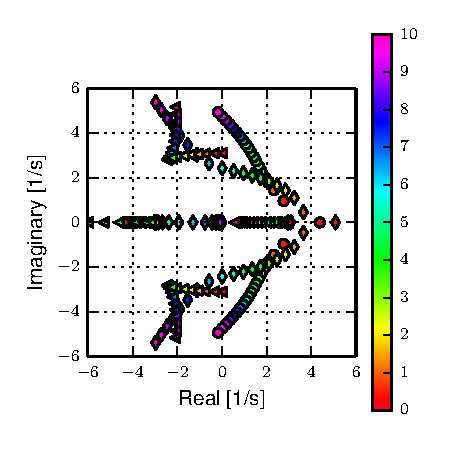
\includegraphics[width=5in]{figures/L-P-rlocus.pdf}
  \caption{Root locus of the identified model (circle), the Whipple model
    (diamond), and the arm model (triangle) with respect to speed in m/s.
    }
\end{figure}

Figure \ref{fig:L-P-eig} gives a different view of the root locus allowing one
to more easily compare the real and imaginary parts of the eigenvalues
independently. The imaginary parts of the weave mode have similar curvature
with respect to speed for all the models about 2m/s or so. The identified model
has a stable speed range where the Whipple model under predicts its weave
critical speed by almost 3 m/s. The identified caster mode is much faster than
that predicted by the Whipple model. This is somewhat counterintuitive
because tire scrub torques would probably tend to slow the caster mode, although 
the pneumatic trail and  arm inertia could play larger
roles than expected.

\begin{figure}
  \label{fig:L-P-eig}
  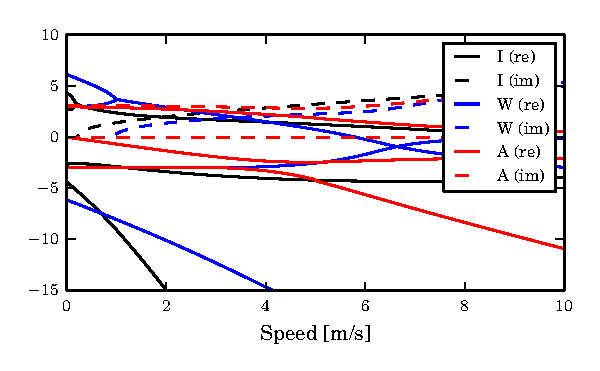
\includegraphics[width=5in]{figures/L-P-eig.pdf}
  \caption{Real and imaginary parts of the eigenvalues as a function of speed
    for model (I)dentified from all runs, the (W)hipple model and the (A)rm
  model.}
\end{figure}

The frequency band from 1 rad/s to 12 rad/s is of most concern as it bounds a
reasonable range that humans operate within. The steer torque
to roll angle transfer function, Figure \ref{fig:L-P-Tdel-Phi} may be the most
important to model accurately as it is the primary method of controlling the
bicycle's direction, i.e. commanding roll allows one to command yaw. At 2 m/s
the magnitude is similar for all three models. At 4 m/s the identified model
has a larger gain than the first principles models. In fact, the identified
model seems to vary little with speed, which contrasts the stronger speed
dependence of the first principles models. The low frequency behavior of the
identified model is not well predicted by the Whipple and arm models at the
three highest speeds but about about 3 rad/s the arm model shows better
magnitude matches than the Whipple model.

\begin{figure}
  \label{fig:L-P-Tdel-Phi}
  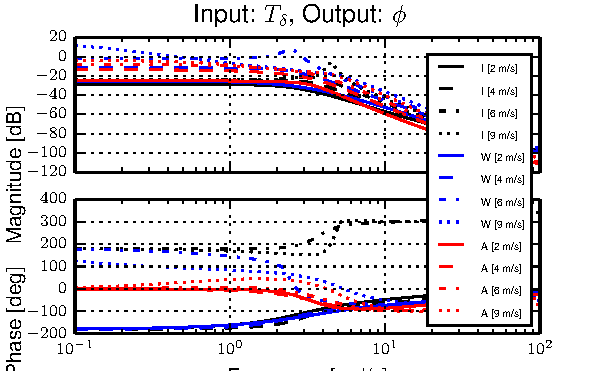
\includegraphics[width=5in]{figures/L-P-Tdel-Phi.pdf}
  \caption{Frequency response of the three models, (I)dentified, (W)hipple, and
    (A)rm, at four speeds (2, 4, 6, and 9 m/s). The color indicates the model
    and the line type indicates the speed}
\end{figure}

Table \ref{tab:L-P-mck} gives the values of the identified coefficients of the
roll and steer equations for the L-P model.

% TODO : Might be a good idea to put an NA in place of the parameters which
% were fixed.
% TODO : Add the arm model some how? Not sure how to compute K0 and K2 quickly,
% needed symbolics in the past.
\begin{table}
  \label{tab:L-P-mck}
  \caption{The identified $\mathbf{M}$, $\mathbf{C}_1$, $\mathbf{K}_0$,
  $\mathbf{K}_2$, and $H$ matrices of the L-P and Whipple
  models.}
  \begin{tabular}{lccccc}
  \toprule
  Model & $\mathbf{M}$ & $\mathbf{C}_1$ & $\mathbf{K}_0$ & $\mathbf{K}_2$ & $H$ \\
  \midrule % \\[0.0625in]
  Whipple &
  $\begin{bmatrix}
    129.362 & 2.260 \\
    2.260 & 0.219 \\
  \end{bmatrix}$
  &
  $\begin{bmatrix}
    0.000 & 41.622 \\
    -0.315 & 1.376 \\
  \end{bmatrix}$
  &
  $\begin{bmatrix}
    -115.707 & -2.361 \\
    -2.361 & -0.737 \\
  \end{bmatrix}$
  &
  $\begin{bmatrix}
    0.000 & 103.943 \\
    0.000 & 2.190 \\
  \end{bmatrix}$
  &
  $\begin{bmatrix}
    0.902 \\
    0.011 \\
  \end{bmatrix}$ \\[0.125in]
  L-P &
  $\begin{bmatrix}
    129.362 & 2.559 \\
    2.559 & 0.250 \\
  \end{bmatrix}$
  &
  $\begin{bmatrix}
    0.000 & 33.526 \\
    -0.549 & 2.100 \\
  \end{bmatrix}$
  &
  $\begin{bmatrix}
    -115.707 & -4.526 \\
    -4.526 & -0.489 \\
  \end{bmatrix}$
  &
  $\begin{bmatrix}
    0.000 & 103.943 \\
    0.000 & 2.603 \\
  \end{bmatrix}$
  &
  $\begin{bmatrix}
    0.902 \\
    0.011 \\
  \end{bmatrix}$\\
  \bottomrule
\end{tabular}

\end{table}

\section{Summary and Acknowledgements}

We have shown that a fourth order linear model is adequate for describing the
motion of the bicycle under manual control in a speed range from approximately
1.5 m/s to 9 m/s. Results from this study show that higher order models may
not be necessary for predicting the bicycle-rider plant dynamics. This is an
important finding, as many researchers develop models using first principles
which have orders much greater than 4, with degrees of freedom associated with
tire slip, frame flexibilities, and rider biomechanics, which may be overkill
for many prediction purposes. But, results also reveal that fourth order
archetypal first principles models are not predictive enough to fully describe
the dynamics. These deficiencies are most likely due to un-modeled effects,
with knife-edge, no side-slip wheel contact assumptions being the most probable
candidate. Un-modeled rider biomechanics such as passive arm stiffness and
damping and head motion may play a role too. It is likely that something as
simple as a ``static'' tire scrub torque is needed to improve the fidelity of
the Whipple first principles derivations, but that doesn't preclude that the
addition of a tire slip model, adding more degrees of freedom, might also
improve the predictive ability.
%\section*{Acknowledgements}
This paper is based on work supported by the National Science Foundation under
Grant No 0928339. Karl {\AA}str{\"o}m provided the ideas for the canonical form.

\bibliographystyle{plain}
\bibliography{references}

\end{document}
